

\begin{frame}{L'IA est complexe !}
  \begin{center}
    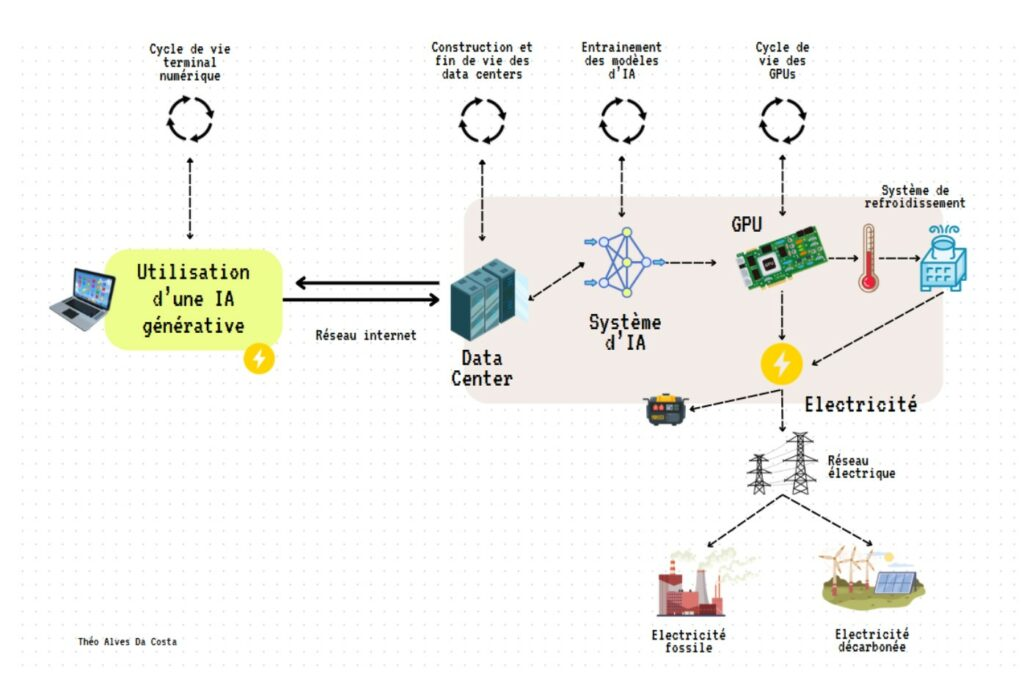
\includegraphics[width=\textwidth]{img/intro/IMAGE-6-credit-Bon-Pote-Theo-Alves-Da-costa-article-IA-1024x682.jpg}
  \end{center}

  {\footnotesize
  Ref : \href{https://bonpote.com/intelligence-artificielle-le-vrai-cout-environnemental-de-la-course-a-lia/}{\underline{Intelligence artificielle : le vrai coût environnemental de la course à l'IA}}}

\end{frame}

\begin{frame}{La donnée au centre !}
  \begin{center}
    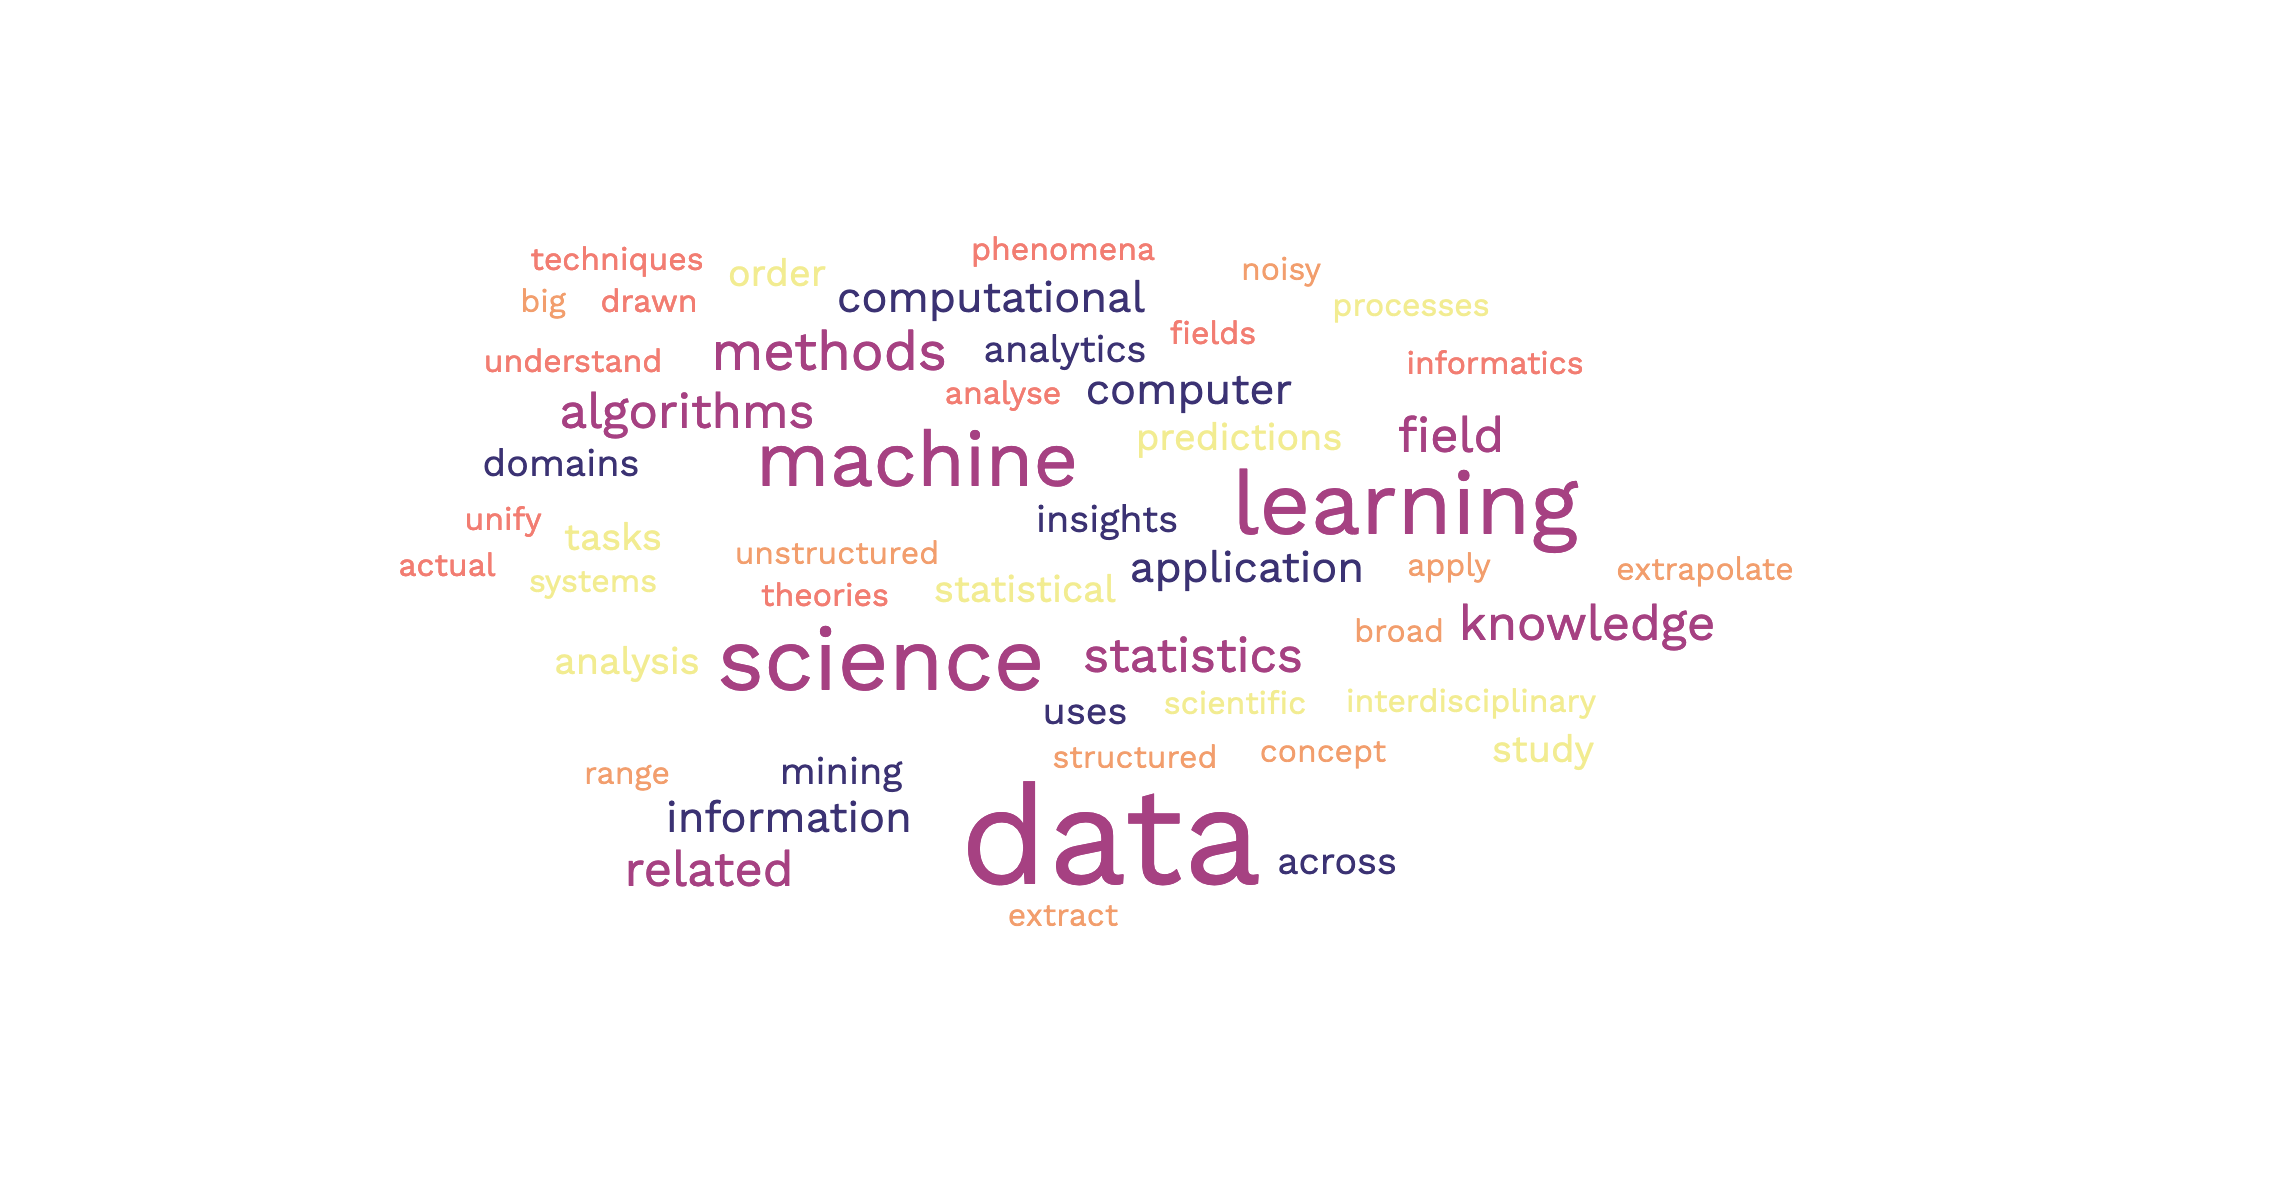
\includegraphics[width=\textwidth]{img/intro/word-cloud.png}
  \end{center}
\end{frame}

\begin{frame}{La donnée au centre !}
  \begin{center}
    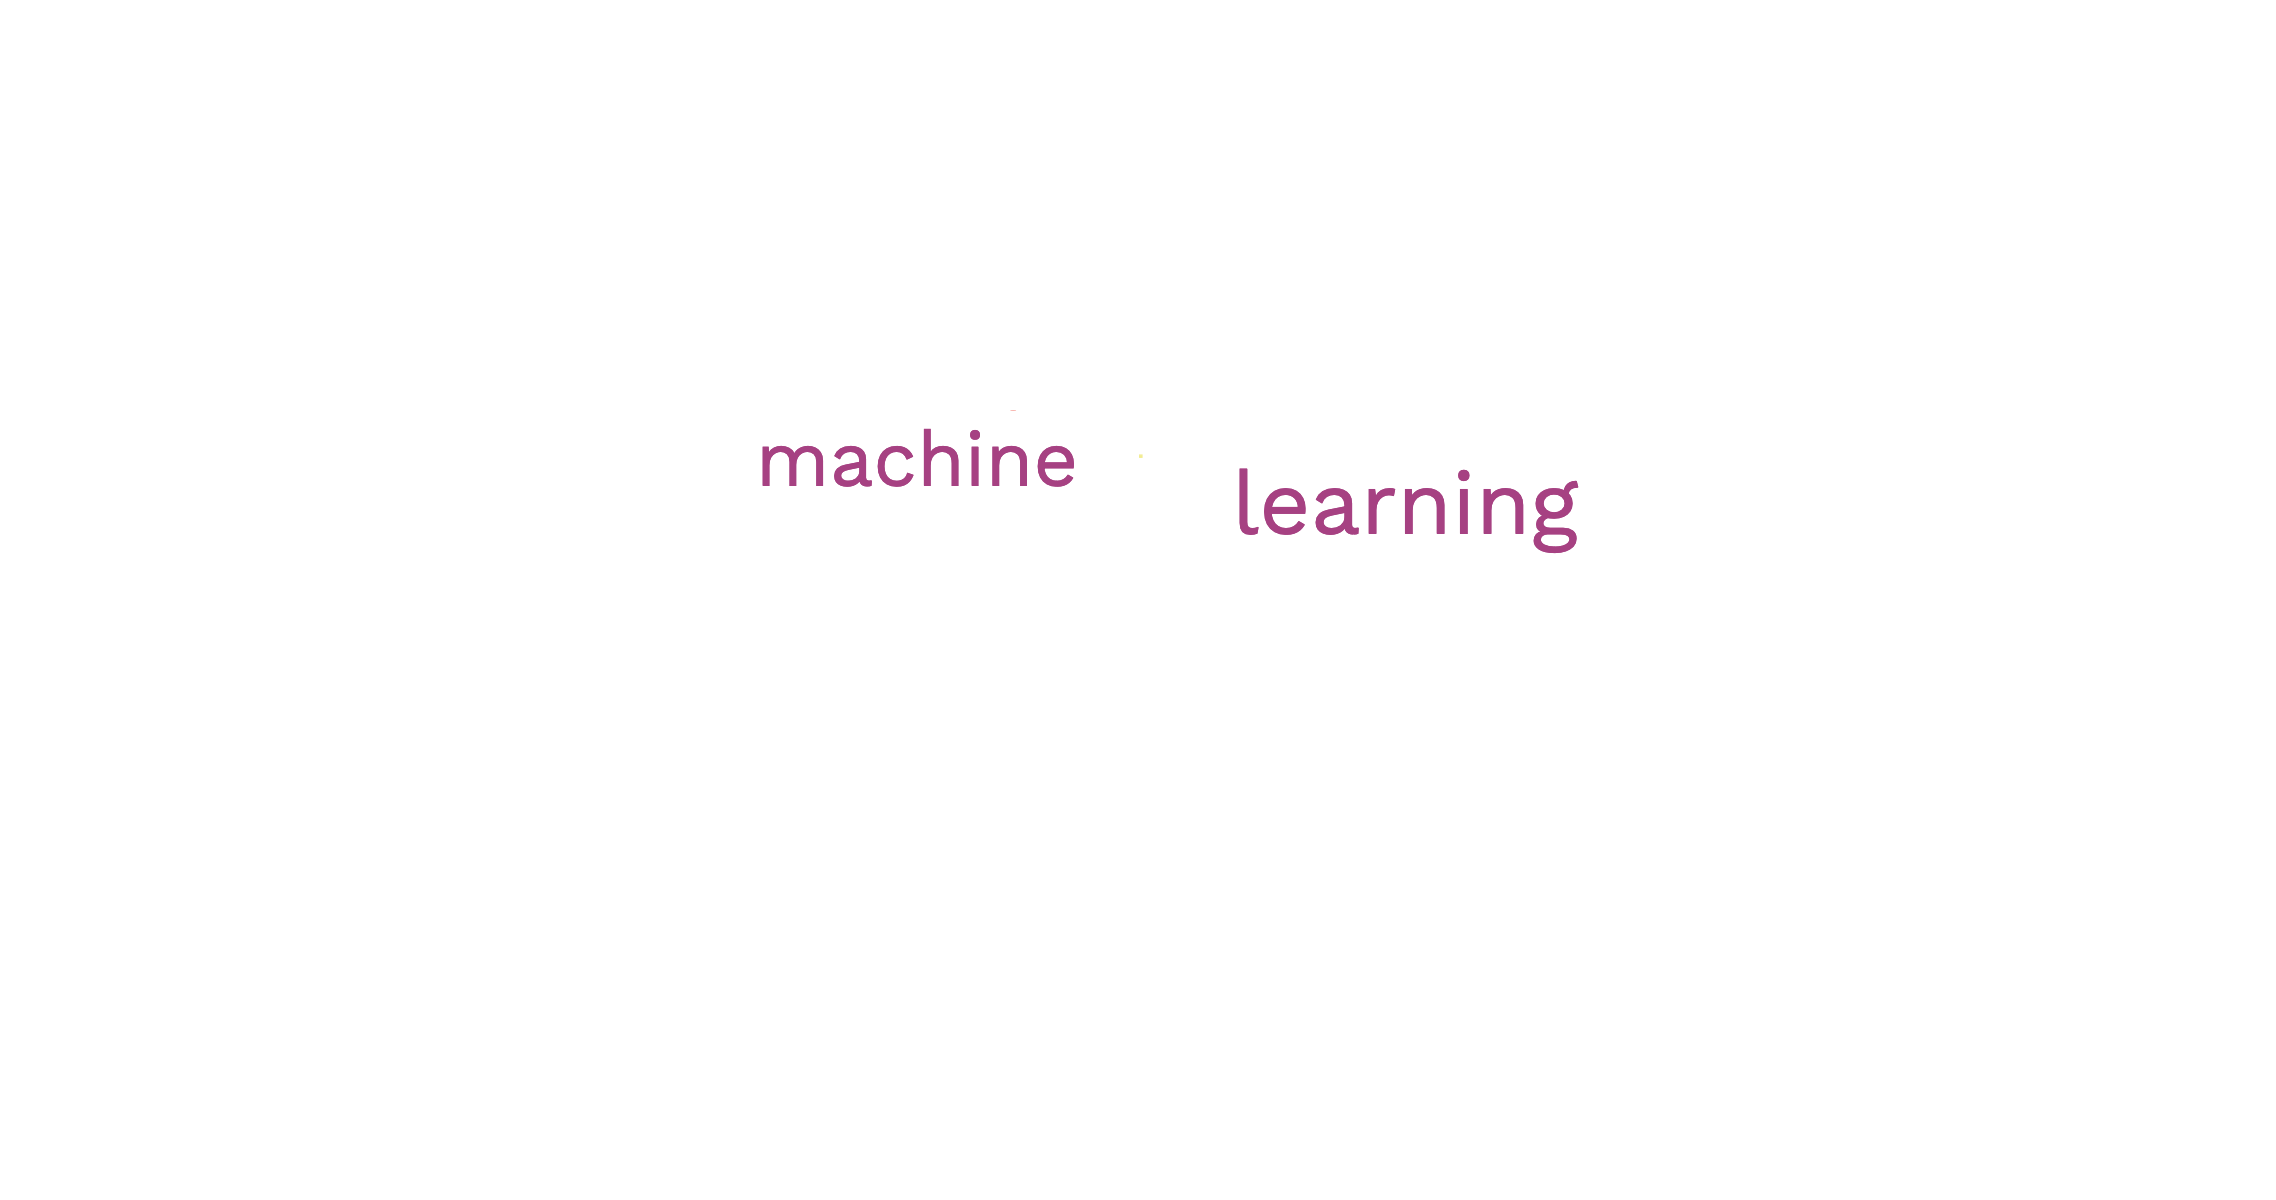
\includegraphics[width=\textwidth]{img/intro/word-cloud-2.png}
  \end{center}
\end{frame}



\section{Données}

\subsection{Data}

\begin{frame}{Qu'est-ce que la donnée ?}
    \begin{center}
        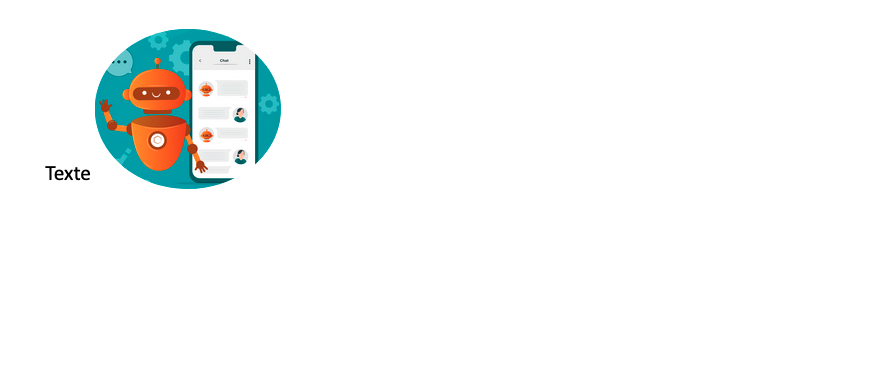
\includegraphics[width=\textwidth]{img/ml/multimodal-1.png}
    \end{center}
\end{frame}

\begin{frame}{Qu'est-ce que la donnée ?}
    \begin{center}
        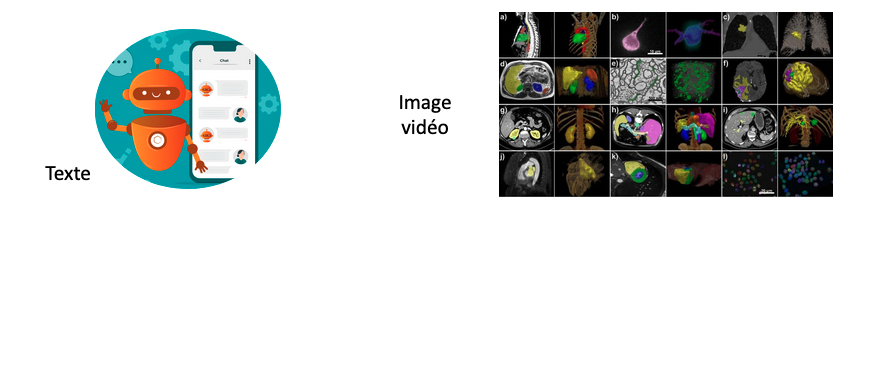
\includegraphics[width=\textwidth]{img/ml/multimodal-2.png}
    \end{center}
\end{frame}

\begin{frame}{Qu'est-ce que la donnée ?}
    \begin{center}
        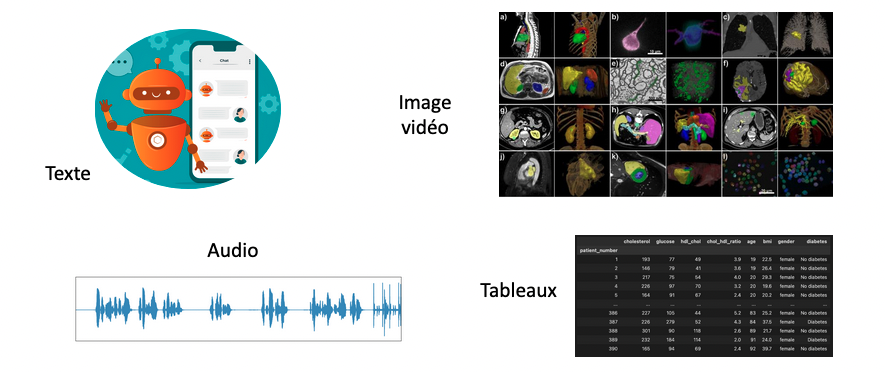
\includegraphics[width=\textwidth]{img/ml/multimodal-3.png}
    \end{center}
\end{frame}


\begin{frame}{Qu'est-ce que la donnée ?}

\textbf{Donnée} = de l'information que l'on peut enregistrer, stocker et analyser

\vspace{0.5cm}

La donnée peut être vue comme une \textbf{observation du monde} (social, physique, etc.).

\medskip

Exemples :
\begin{itemize}
    \item Produits : \textit{``Produit X, \$29.99, 1000 unités achetée en 2025''}
    \item Santé des patients : \textit{``Température 38°C, pression artérielle 120/80''}
    \item Une photo : \textit{``Ciel bleu, deux personnes, extérieur''}
\end{itemize}

\vspace{0.5cm}

\end{frame}

\begin{frame}{Trois types de données}

\begin{columns}[T]
\begin{column}{0.33\textwidth}
    \centering
    \textbf{Données tabulaires}\\
    \vspace{0.3cm}
    Structurées en lignes \& colonnes\\
    \vspace{0.2cm}
    \small Comme dans des tableurs
\end{column}

\begin{column}{0.33\textwidth}
    \centering
    \textbf{Images}\\
    \vspace{0.3cm}
    Information visuelle\\
    \vspace{0.2cm}
    \small Photos, dessins, scans
\end{column}

\begin{column}{0.33\textwidth}
    \centering
    \textbf{Données textuelles}\\
    \vspace{0.3cm}
    Langage naturel, écrit\\
    \vspace{0.2cm}
    \small Documents, emails, textes historiques
\end{column}
\end{columns}

\vspace{1cm}

\textbf{Chaque type de données correspond à des cas d'usage spécifiques}

\end{frame}



\begin{frame}
\frametitle{Type 1 : Données tabulaires}

\textbf{Qu'est-ce que c'est ?} L'information est organisée en un tableau
 
\vspace{0.5cm}

\textbf{Exemple: base de données clients}

\begin{table}
\small
\begin{tabular}{|l|c|c|c|}
\hline
\textbf{Name} & \textbf{Age} & \textbf{City} & \textbf{Purchase} \\
\hline
Alice & 32 & Paris & \$150 \\
Bob & 28 & Lyon & \$75 \\
Carol & 45 & Marseille & \$200 \\
\hline
\end{tabular}
\end{table}

\vspace{0.5cm}

\textbf{Chaque ligne} = une personne (ou produit, transaction, etc.)\\
\textbf{Chaque colonne} = une caractéristique

\vspace{0.3cm}

\textbf{Cas d'usage :} Predire le comportement client, recommender des produits

\end{frame}

\begin{frame}{Type 2 : image}

\textbf{Qu'est-ce que c'est ?} Photos, dessins, scans, screenshots

\vspace{0.5cm}

\begin{columns}
\begin{column}{0.5\textwidth}
    \textbf{Que voit un humain :}
    \begin{itemize}
        \item Un chat dans une combinaison spatiale
        \item Une bouteille dans un desert
    \end{itemize}
\end{column}

\begin{column}{0.5\textwidth}

  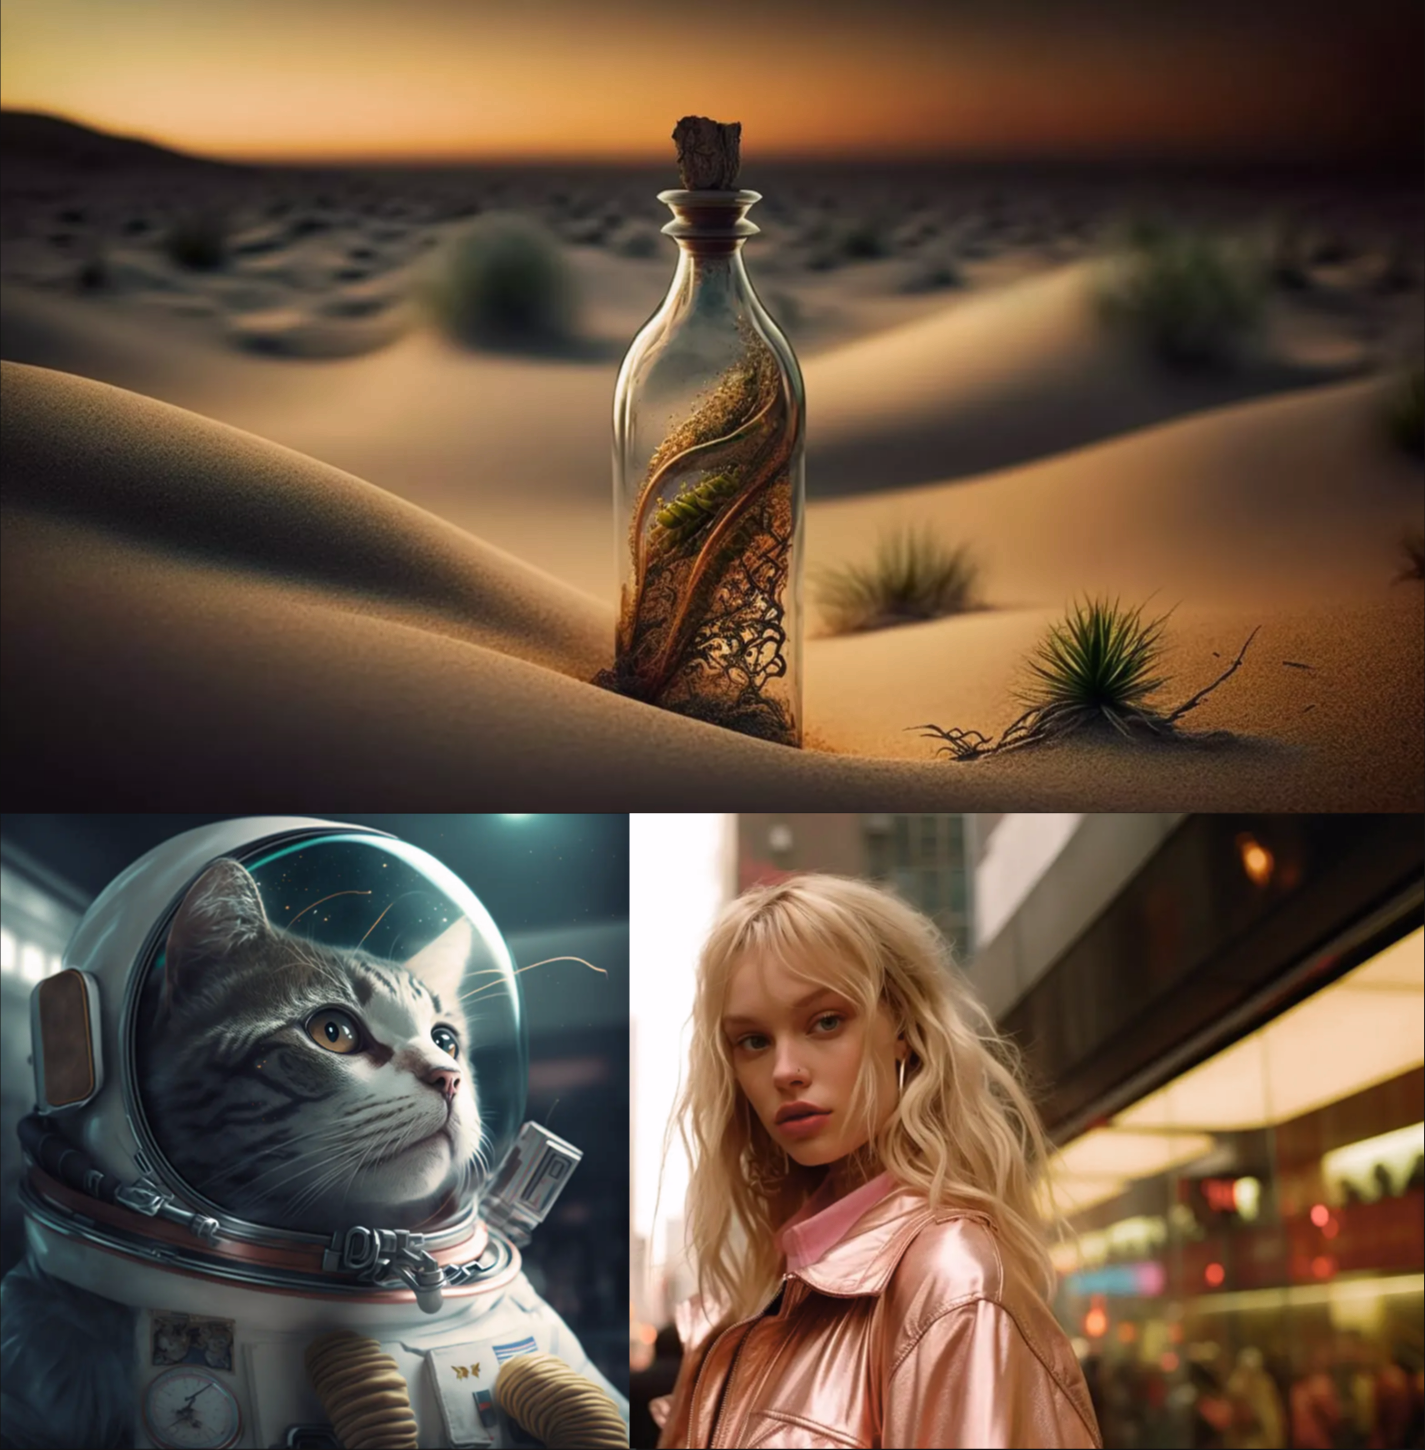
\includegraphics[width=.5\textwidth]{img/intro/midjourney.png}

\end{column}
\end{columns}

\vspace{0.5cm}

\textbf{Cas d'usage :} Détection d'objets / forme, diagnostics médicaux

\end{frame}




\begin{frame}{Type 2 : image}

\textbf{Qu'est-ce que c'est ?} Photos, dessins, scans, screenshots

\vspace{0.5cm}

\begin{columns}
\begin{column}{0.5\textwidth}
    \textbf{Que voit un humain :}
    \begin{itemize}
        \item Un chat dans une combinaison spatiale
        \item Une bouteille dans un desert
    \end{itemize}
\end{column}

\begin{column}{0.5\textwidth}

  \textbf{Que voit un ordinateur :}
  \begin{itemize}
      \item Des millions de points (pixels)
      \item Chaque pixel correspond à une couleur spécifique
      \item Structure en grille RGB
  \end{itemize}
\end{column}
\end{columns}

\vspace{0.5cm}

\textbf{Cas d'usage :} Détection d'objets / forme, diagnostics médicaux

\end{frame}



\begin{frame}{Type 2 : image}

\textbf{Définition :} un tableau 3D, chaque pixel contenant une valeur numérique

\vspace{0.3cm}

\begin{center}
  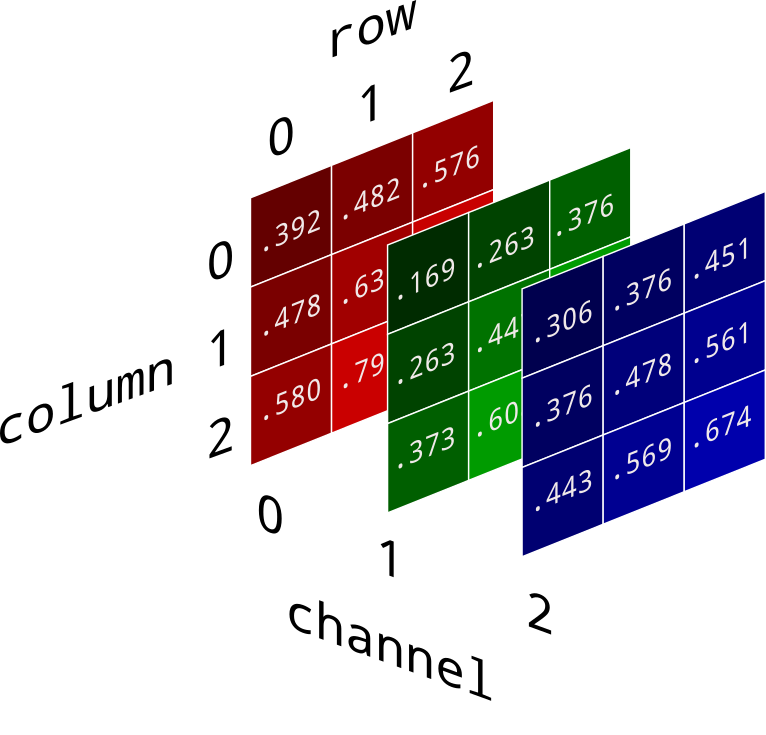
\includegraphics[width=.4\textwidth]{img/intro/rgb.png}
\end{center}

\vspace{0.3cm}

\textbf{Ordre de grandeurs :}
\begin{itemize}
  \item Image 224 x 224 pixels = 224 x 224 x 3 = 150 528 valeurs
  \item Photo 20M pixels = 5500 x 3700 x 3 = +60M valeurs
\end{itemize}

\end{frame}


\begin{frame}{Type 3 : données textuelles}

\textbf{Qu'est-ce que c'est ?} Contenu écrit, langage

\vspace{0.5cm}

\textbf{Exemples :}
\begin{itemize}
    \item Commentaires clients : \textit{``Super produit, envoi rapide !''}
    \item Réseaux sociaux, emails : \textit{``Just had the best coffee :-)''}
    \item Documents : contrats, raports, articles
\end{itemize}

\vspace{0.5cm}

\textbf{Challenge:} Le langage est ambigu, contextuel et créatif
\begin{itemize}
    \item ``banque'' = organisation financière ou médicale ?
    \item Sarcasme: ``Super, une autre réunion !''
\end{itemize}

\vspace{0.3cm}

\textbf{Cas d'usage :} Analyse de sentiments, traduction, chatbots

\end{frame}


\begin{frame}{Type 3 : données textuelles}

\textbf{Définition :} Séquences de symboles (caractères, mots, tokens)

\vspace{0.3cm}

\colorwarning{red}\textbf{Challenge :} les ordinateur traitent des nombres mais pas des mots

\vspace{0.3cm}

\textbf{Besoin de transformer les mots en nombres :}

\begin{enumerate}
    \item \textbf{Niveau ``caractère''} : chaque caractère remplacé par des nombres distincts
        \begin{itemize}
            \item[\textcolor{white}{x}] ``cat'' → [99, 97, 116]
        \end{itemize}
    
    \item \textbf{Niveau ``mot''} : encoder les mots (ou les sous-mot)
        \begin{itemize}
          \item[\textcolor{white}{x}] Word embeddings : chaque mot est un vector de nombres
          \item[\textcolor{white}{x}] → Nécessite la connaissance de l'ensemble des mots
        \end{itemize}
\end{enumerate}

\end{frame}




\begin{frame}{Trois types de données : approches différentes}

Différents type de données nécessitent \textbf{différentes approches IA}:

\vspace{0.5cm}

\begin{tabular}{l|l|l}
\textbf{Type} & \textbf{Approche} & \textbf{Dimensionnalité}\\
\hline
Tabulaire & Modèles statistiques & \textcolor{blue}{Modérée}\\
          & arbres de décision   & 10-1000 variables \\
Image & Vision par ordinateur    & \textcolor{red}{Très grande}\\
      & réseaux de neurones      & 100k-70M valeurs\\
Texte & Traitement automatique   & \textcolor{orange}{Grande}\\
      & du langage (NLP)         & 50k-100k mots\\
\end{tabular}

\onslide<2>
\colorwarning{orange}Les LLMs sont construits sur des \textcolor{red}{tokens} et pas uniquement sur des mots. La dimensionnalité peut atteindre des trillions !

\end{frame}

\begin{frame}{Trois types de données : approches différentes}

    \onslide<1->

      \textbf{Modèle tabulaire}
      \bigskip

      \begin{center}
        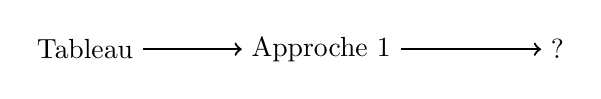
\begin{tikzpicture}[
          every node/.style={align=center},
          arrow/.style={->, thick}
        ]
          \node (table) at (-3,0) {Tableau};
          
          % Box in the middle
          \node (box) at (0,0) {\boxed{\mbox{Approche 1}}};
          
          % Text on the right
          \node (right) at (3,0) {?};
          
          % Arrows
          \draw[arrow] (table) -- (box);
          \draw[arrow] (box) -- (right);
        \end{tikzpicture}
      \end{center}

    \onslide<2->
      \textbf{Modèle de vision par ordinateur}
      \bigskip

      \begin{center}
        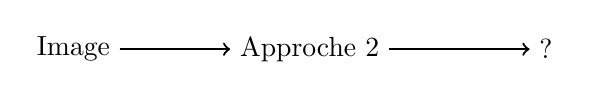
\begin{tikzpicture}[
          every node/.style={align=center},
          arrow/.style={->, thick}
        ]
          \node (image) at (-3,0) {Image};
          
          % Box in the middle
          \node (box) at (0,0) {\boxed{\mbox{Approche 2}}};
          
          % Text on the right
          \node (right) at (3,0) {?};
          
          % Arrows
          \draw[arrow] (image) -- (box);
          \draw[arrow] (box) -- (right);
        \end{tikzpicture}
      \end{center}
    \onslide<3>
      \textbf{Modèle de NLP}
      \bigskip
      
      \begin{center}
        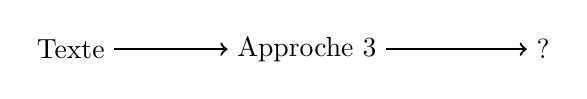
\begin{tikzpicture}[
          every node/.style={align=center},
          arrow/.style={->, thick}
        ]
          \node (text) at (-3,0) {Texte};
          
          % Box in the middle
          \node (box) at (0,0) {\boxed{\mbox{Approche 3}}};
          
          % Text on the right
          \node (right) at (3,0) {?};
          
          % Arrows
          \draw[arrow] (text) -- (box);
          \draw[arrow] (box) -- (right);
        \end{tikzpicture}
      \end{center}

\end{frame}

\begin{frame}{Trois types de données : approches différentes}

      \textbf{Modèle \textcolor{red}{multimodal}}
      \bigskip
      
      \begin{center}
        \begin{tikzpicture}[
          every node/.style={align=center},
          arrow/.style={->, thick}
        ]
          \node (text) at (-3,-2) {Tableau};
          \node (image) at (-3,0) {Image};
          \node (table) at (-3,2) {Texte};
          
          % Box in the middle
          \node (box) at (0,0) {\boxed{\mbox{Approche 4}}};
          
          % Text on the right
          \node (right) at (3,0) {?};
          
          % Arrows
          \draw[arrow] (table) -- (box);
          \draw[arrow] (image) -- (box);
          \draw[arrow] (text) -- (box);
          \draw[arrow] (box) -- (right);
        \end{tikzpicture}
      \end{center}
  
\end{frame}

